\documentclass[a4paper,fontsize=14pt]{article}
\usepackage[left=3cm, right=1.5cm, top=2cm, bottom=2cm, nohead, bindingoffset=0cm]{geometry}
%\usepackage[left=20mm, top=15mm, right=15mm, bottom=15mm, nohead, footskip=10mm]{geometry} % settings of fields colors

% input document encoding
\usepackage[utf8]{inputenc}

% support of Russian letters
% font encoding
\usepackage[T2A]{fontenc}

% package for use of Russian letters in formulas
\usepackage{amsmath, amsfonts}

% setting the one-and-a-half interval
\usepackage{setspace}  
\onehalfspacing

% use Times New Roman but disable text highlightning
%\renewcommand{\rmdefault}{ftm}

% languages used in the article 
% + the ability to correctly hyphenate words
\usepackage[english,russian]{babel}
\usepackage{cmap}

% packages for references and hyperreferences.
\usepackage{xcolor}
\definecolor{commentgreen}{RGB}{2,112,10}
\definecolor{eminence}{RGB}{108,48,130}
\definecolor{weborange}{RGB}{255,165,0}
\definecolor{frenchplum}{RGB}{129,20,83}

\usepackage{caption}

% improve citations handling
\usepackage{cite}

% hyperreference colors
\usepackage{hyperref}
%\definecolor{linkcolor}{HTML}{799B03} % reference color
%\definecolor{urlcolor}{HTML}{799B03} % hyperreference color
%\hypersetup{pdfstartview=FitH, linkcolor=linkcolor, urlcolor=urlcolor, colorlinks=true}

% picture packages
\usepackage{graphicx}
\graphicspath{{pictures/}}
\DeclareGraphicsExtensions{.pdf,.png,.jpg}

% place pictuire exactly to the specified location
\usepackage{flafter}

% use to highlight text
\usepackage{ulem}

% add references to the table of content page
\usepackage[nottoc]{tocbibind}

% indent the first paragraph of a Chapter or paragraph
\usepackage{indentfirst}

% set specific options to sections and subsections
\usepackage{titlesec}
% set the font size for sections
\titleformat*{\section}{\fontsize{18pt}{18pt}\selectfont\bfseries\filcenter}
\titleformat*{\subsection}{\fontsize{16pt}{18pt}\selectfont\bfseries\filcenter}
% add dot after section number
%\titlelabel{\thetitle.\quad}

% start every section with new page
\newcommand{\sectionbreak}{\clearpage}

% use predefined text number char
\newcommand*{\No}{\textnumero}

\begin{document}
% set the font size for the entire document
\fontsize{14pt}{18pt}\selectfont

\hyphenation{SPbU}

\author{Vasilyev~V.\:V., Nikiforov~K.\:A.}
\title{Application of probabilistic analysis to the problem of finding the shortest route}

%\renewcommand{\thefootnote}{ }
%{\footnotetext{{\it E"=mail addresses} : vasar007@yandex.ru (Vasilyev~V.\:V.), k.nikiforov@spbu.ru (Nikiforov~K.\:A.)}}

%\date{01.12.2019}

% НАЧАЛО ТИТУЛЬНОГО ЛИСТА
\begin{center}
	\large{САНКТ"=ПЕТЕРБУРГСКИЙ ГОСУДАРСТВЕННЫЙ УНИВЕРСИТЕТ}\\ 
	\large{02.03.02 <<Фундаментальная информатика и информационные технологии>>}\\
	\large{ООП: Программирование и информационные технологии}\\

	\hfill \break
	\hfill \break
	\hfill \break
	\hfill \break
	
	\large{\textbf{ОТЧЕТ О НАУЧНО"=ИССЛЕДОВАТЕЛЬСКОЙ РАБОТЕ}}\\
\end{center}

\begin{flushleft}
	\begin{large}
		\hfill \break
		\textbf{Тема задания: \uline{Оценка трудоемкости алгоритма на основе эмпирического анализа}} \\
		\hfill \break
		\textbf{Выполнил:} $\underset{\text{Фамилия~И.\:О.}}{\text{\uline{\hspace{7em} \textbf{Васильев~В.\:В.}\hspace{7em}}}}$ $\underset{\text{номер группы}}{\text{\uline{16.Б13"=пу}}}$ \\
		\hfill \break
		\textbf{Руководитель научно"= \\[-2ex]
			исследовательской работы:} $\underset{\text{ФИО, должность, ученая степень}}{\text{\uline{\hspace{7em} Никифоров~К.\:А., \hspace{7em}}}}$ \uline{кандидат физ.--мат. наук, доцент}
	\end{large}
\end{flushleft}

\hfill \break
\hfill \break
\hfill \break
\hfill \break
\hfill \break
\hfill \break
\hfill \break
\hfill \break
\hfill \break
\hfill \break
\hfill \break
\hfill \break
\hfill \break
\hfill \break
\hfill \break
\hfill \break

\begin{center} Санкт"=Петербург, 2019 \end{center}
\thispagestyle{empty} % выключаем отображение номера для этой страницы

% КОНЕЦ ТИТУЛЬНОГО ЛИСТА

\newpage

\tableofcontents

\newpage

\section{Введение} \label{sec:introduction}

Одним из ключевых свойств алгоритма является его эффективность. Это свойство связано с вычислительными ресурсами, используемыми алгоритмом. В настоящее время наиболее широко используемой оценкой является функция сложности в среднем, на основе которой с достаточно хорошей точностью могут быть прогнозированы (в статистическом смысле) временные оценки программной реализации алгоритма.

Однако проблема заключается в том, что средняя оценка, будучи статистической и точечной, не дает никакой информации о поведении алгоритма на конкретных входах, что важно как для задач большой размерности, так и для систем реального времени. Использование оценки в худшем случае приводит к существенному завышению временного прогноза из"=за малой вероятности входных данных, обеспечивающих максимум функции трудоемкости алгоритма при фиксированной размерности задачи. Таким образом, интерес представляет задача построения практически значимой интервальной оценки трудоемкости алгоритма.

% TODO: переписать этот абзац (текст не уникальный).
Возможным решением задачи повышения точности результатов эмпирического анализа алгоритма является рассмотрение функции трудоемкости при фиксированной входной длине как дискретной ограниченной случайной величины, имеющей некоторое неизвестное распределение. Подход заключается в построении доверительного интервала трудоемкости на основе аппроксимации неизвестного дискретного распределения значений трудоемкости непрерывным распределением с ограниченной вариацией, для чего предлагается использовать бета"=распределение. Полученное решение позволяет задать более реальную правую границу сложности алгоритма при фиксированной входной длине с заданной доверительной вероятностью.

% TODO: переписать этот абзац (текст не уникальный).
Данный метод включает в себя два этапа. Первый этап~--- предварительное исследование, целью которого является проверка гипотезы о виде закона распределения значений трудоемкости алгоритма как дискретной ограниченной случайной величины~\cite{petrushyn_ulyanov_planning}. Второй этап~--- основное исследование,в ходе которого значения доверительной трудоемкости $f_\gamma(n)$ определяются в зависимости от входной длины алгоритма~\cite{petrushyn_ulyanov_analysis}.

\section{Постановка задачи} \label{sec:problem_statement}

Целью данной работы является исследование применимости вероятностного анализа функции трудоемкости алгоритма и сравнение полученных результатов с классическим эмпирическим подходом. Основными задачами являются:

\begin{enumerate}
	\item[•] выбор алгоритма для анализа;

	\item[•] реализация выбранного алгоритма и генератора входных данных на одном из языков программирования;

	\item[•] проведение этапа предварительного исследования и рассмотрение гипотезы о выбранном распределении;

	\item[•] в случае принятия гипотезы о распределении проведение этапа основного исследования и выявление зависимости доверительной трудоемкости от входной длины алгоритма;
	
	\item[•] анализ полученных результатов.
\end{enumerate}

В качестве алгоритма исследования возьмем один из алгоритмов нахождения кратчайших путей в графе~--- алгоритм Паллоттино.

\section{Описание выбранного алгоритма} \label{sec:pallotino_algorithm}

Нахождение кратчайшего пути от одной вершины до всех остальных является одной из основных задач оптимизации сети. Существует несколько распространенных и хорошо известных алгоритмов, которые решают эту проблему. Одна категория состоит из алгоритма Дейкстры~\cite{dijkstra} и его модификаций, другая категория содержит алгоритм Беллмана\,--\,Форда\,--\,Мура~\cite{bellman, ford, moore} и его модификации. Есть также ряд других алгоритмов, которые не входят в эти категории. Однако они не будут рассмотрены в силу невозможности охватить всевозможные алгоритмы нахождения кратчайших путей в одной работе.

Алгоритм Паллоттино~--- алгоритм, который находит кратчайшее расстояние от одной из вершин до всех остальных на графах без петель, является модификацией алгоритма Беллмана\,--\,Форда\,--\,Мура. Этот алгоритм также работает для графов с ребрами отрицательного веса при определенных условиях. Он широко используется для решения задач оптимального распределения грузопотоков по транспортной сети и выбора наиболее выгодных путей ее развития.

В литературе есть небольшая путаница с наименованием этого алгоритма. Пейп развил предложение Д'Эсопо~\cite{desopo} и предложил улучшенный алгоритм~\cite{pape}. В то же время Левит и Лившиц разработали свою версию с той же идеей~\cite{levit_livshits}. Таким образом, у нас есть алгоритм Д'Эсопо\,--\,Пейпа\,--\,Левита, который использует двухстороннюю очередь для поддержания помеченных вершин в графе. Позже Паллоттино предложил использовать две очереди вместо двухсторонней очереди, чтобы избежать экспоненциальной сложности алгоритма~\cite{pallottino}. Именно последний алгоритм является объектом исследований в данной работе.

Входными данными для алгоритма является граф $G$, подаваемый в виде упорядоченной совокупности множеств вершин $V$ и ребер $E$: $G = (V, E)$. Оценка размера входных данных производится по размеру множеств вершин и ребер. Пусть $n$~--- количество вершин в множестве $V$, $m$~--- количество ребер в множестве $E$: $n = |V|, m = |E|$. В качестве основной операции алгоритма выберем операцию релаксации ребра.

% TODO: релазиовать генератор географических графов и обновить текст (и граф реальных географических дорог Санкт-Петербурга).
Для анализа алгоритма Паллоттино был использован генератор полных графов без мультиребер. Стоит отметить, что генератор входных данных должен обеспечивать репрезентативность выборки, т.~е. генерировать такие входные данные, которые по вероятности соответствуют особенностям применения данного алгоритма. Поскольку алгоритм Паллоттино используется для решения транспортных задач, в реализацию генератора было добавлено условие: для любых трех узлов графа должно выполняться неравенство треугольника. Пусть $G = (V, E)$~--- полный неориентированный граф с $n$ вершинами, $W: E \rightarrow R_+$~--- функция весов ребер. Тогда неравенство треугольника имеет вид:

\begin{equation}\label{eq:triangle_inequality}
W((u, w)) \leq W((v, u)) + W((u, w)), \forall u, v, w \in V.
\end{equation}

Отметим, что алгоритм Паллотино имеет оценки

\begin{equation}\label{eq:pallottino_best}
O(n, m) = n,
\end{equation}

\begin{equation}\label{eq:pallottino_average}
O(n, m) = n \cdot m,
\end{equation}

\begin{equation}\label{eq:pallottino_worst}
O(n, m) = n^2 \cdot m
\end{equation}

в лучшем, среднем и худшем случаях соответственно~\cite{pallottino}.

\section{Этап предварительного исследования} \label{sec:analysis_part_1}

\subsection{Основные этапы} \label{subsec:analysis_part_1_intro}

Организация экспериментального исследования сложности алгоритма привела к необходимости модификации исходного кода реализации алгоритма Паллоттино, связанной с размещением счетчика для определения значения числа выполняемых основных операций на этом входе.

Рассмотрим более подробно этап планирования предварительного исследования~\cite{petrushyn_ulyanov_planning}. Основной задачей этого этапа является определение рационального размера выборки при фиксированной длине входа для проведения экспериментальных исследований трудоемкости алгоритма в среднем. Все формулы для расчетов взяты из методики~\cite{petrushyn_ulyanov_planning}.

Выдвигается гипотеза, что функция трудоемкости алгоритма Паллоттино имеет бета"=распределение. Основные этапы предварительного исследования:

\begin{enumerate}
	\item Фиксация некоторого значения длины входа $n$ из реального сегмента длин в области применения алгоритма Паллоттино. В рассматриваемом случае $n = 80$.
	
	\item Определение необходимого числа экспериментов $m$ с программной реализацией для получения гистограммы относительных частот значений трудоемкости, например, по методике, изложенной в~\cite{petrushyn_ulyanov_planning}.
	
	\item Проведение экспериментального исследования и получение значений трудоемкости $f_i$ для сгенерированных случайных допустимых входов $D_i$: $f_i = f_A(D_i), i = \overline{1, m}$, где $f_A(D_i)$~--- произвольное значение функции трудоемкости.
	
	\item Получение теоретических функций трудоемкости алгоритма для лучшего и худшего случаев, как функций длины входа. Для алгоритма Паллоттино эти функции имеют вид:
	
	\begin{equation}\label{eq:complexity_function_1}
	f_A^\vee(n) = n,
	\end{equation}
	
	\begin{equation}\label{eq:complexity_function_2}
	f_A^\wedge(n) = {n^3 \cdot (n - 1) \over{2}}.
	\end{equation}
	
	Последняя формула следует из того, что алгоритм Паллоттино в худшем случае имеет оценку (\ref{eq:pallottino_worst}), а поскольку для полных графов \\ $m = {n \cdot (n - 1) \over{2}}$, получаем (\ref{eq:complexity_function_2}).
	
	\item Выбор числа $s$ полусегментов для гистограммы частот значений трудоемкости.
	
	\item Нормирование значений экспериментальной трудоемкости и построение на основе полученных данных гистограммы относительных частот в полусегментах.
	
	\item Вычисление нормированного выборочного среднего и нормированной исправленной выборочной дисперсии по формулам:
	
	\begin{equation}\label{eq:mean}
	\overline{t} = {\overline{f_t}(n) - f^\wedge \over{f^\wedge - f^\vee}},
	\end{equation}
	
	\begin{equation}\label{eq:variance}
	s^2 = {1 \over{m - 1}} \sum_{i=1}^{m} {(f_i - \overline{f_t}(n))^2 \over{(f^\wedge - f^\vee)^2}},
	\end{equation}
	
	где $f^\wedge$ и $f^\vee$~--- соответственно максимальное и минимальное значение теоретических функций трудоемкости, $\overline{f_t}(n)$~--- выборочное среднее.
	
	\item Формулировка гипотезы и расчет параметров аппроксимирующего закона распределения. В данном случае выдвигается гипотеза о бета"=распределении. Параметры бета"=распределения рассчитываются по формулам:
	
	\begin{equation}\label{eq:alpha}
	\alpha = {\overline{t} \over{s^2}} (\overline{t} - (\overline{t})^2 - s^2),
	\end{equation}
	
	\begin{equation}\label{eq:beta}
	\beta = {(1 - \overline{t}) \over{s^2}} (\overline{t} - (\overline{t})^2 - s^2).
	\end{equation}
	
	\item Расчет теоретических частот по функции плотности по формуле:
	
	\begin{equation}\label{eq:frequency}
	p_i = \int_{x_i}^{x_i + \Delta x_i} b(x, \alpha, \beta) dx,
	\end{equation}
	
	где $b$~--- функция бета"=распределения.
	
	\item Расчет наблюдаемого значения критерия Пирсона по формуле:
	
	\begin{equation}\label{eq:pirson_criteria}
	\chi_{\text{набл}}^2 = m \sum_{i=1}^{s} {(w_i - p_i)^2 \over{p_i}},
	\end{equation}
	
	где $w_i$~--- относительные частоты.
	
	\item Проверка гипотезы о законе распределения. Если нет оснований отвергнуть нулевую гипотезу, то переход к основному этапу исследования. В противном случае – выбор другого закона распределения и повторная проверка гипотезы.
\end{enumerate}

\subsection{Результаты предварительного исследования} \label{subsec:results_part_1}

Для оценки необходимого числа экспериментов с программной реализацией алгоритма Паллоттино для фиксированной длины входа ($n = 80$) в соответствие с изложенной методикой был проведен этап предварительного исследования с коэффициентом доверия $\gamma = 0.95$.

Сначала была извлечена выборка объемом 200, вычислен коэффициент вариации $V_f = {\sigma^2 \over{\overline{t}}}$, вычислено значение $m_{(1)}^*$, результаты приведены в таблице 1.

\begin{center}
	\label{table1}
	Таблица 1 \\
	\hfill \break
	\begin{tabular}{|c|c|}
		\hline
		Предварительный объем выборки & 200 \\
		\hline
		Выборочное среднее & 9372.87 \\
		\hline
		Выборочная дисперсия & 2774677.39005 \\
		\hline
		Выборочное отклонение & 1665.736291 \\
		\hline
		Коэффициент вариации & 0.177718915 \\
		\hline
		Рассчитанный объем выборки & 121334 \\
		\hline
	\end{tabular}
\end{center}

Далее была извлечена выборка объемом 121334, результаты ее обработки приведены в таблице 2. Поскольку рассчитанный объем выборки оказался больше, чем объем выборки текущего эксперимента, то $m_{(1)}^* = 148178$.

\begin{center}
	\label{table2}
	Таблица 2 \\
	\hfill \break
	\begin{tabular}{|c|c|}
		\hline
		Предварительный объем выборки & 121334 \\
		\hline
		Выборочное среднее & 9524.10 \\
		\hline
		Выборочная дисперсия & 3498806.02004 \\
		\hline
		Выборочное отклонение & 1870.509562 \\
		\hline
		Коэффициент вариации & 0.1963974169 \\
		\hline
		Рассчитанный объем выборки & 148178 \\
		\hline
	\end{tabular}
\end{center}

Далее была извлечена выборка объемом 148178, результаты ее обработки приведены в таблице 3. Поскольку рассчитанный объем выборки оказался больше, чем объем выборки текущего эксперимента, то $m_{(1)}^* = 149628$.

\begin{center}
	\label{table3}
	Таблица 3 \\
	\hfill \break
	\begin{tabular}{|c|c|}
		\hline
		Предварительный объем выборки & 148178 \\
		\hline
		Выборочное среднее & 9531.38 \\
		\hline
		Выборочная дисперсия & 3538446.02776 \\
		\hline
		Выборочное отклонение & 1881.075763 \\
		\hline
		Коэффициент вариации & 0.197356002 \\
		\hline
		Рассчитанный объем выборки & 149628 \\
		\hline
	\end{tabular}
\end{center}

Далее была извлечена выборка объемом 149628, результаты ее обработки приведены в таблице 4. Поскольку рассчитанный объем выборки оказался меньше, чем объем выборки текущего эксперимента, то $m = 149192$.

\begin{center}
	\label{table4}
	Таблица 4 \\
	\hfill \break
	\begin{tabular}{|c|c|}
		\hline
		Предварительный объем выборки & 149628 \\
		\hline
		Выборочное среднее & 9526.48 \\
		\hline
		Выборочная дисперсия & 3524490.40991 \\
		\hline
		Выборочное отклонение & 1877.362621 \\
		\hline
		Коэффициент вариации & 0.197067772 \\
		\hline
		Рассчитанный объем выборки & 149192 \\
		\hline
	\end{tabular}
\end{center}

Далее была извлечена итоговая выборка объемом 149192 и построена гистограмма относительных частот на 387 полусегментах. Данное значение для количества полусегментов было получено с помощью функции создания гистограммы относительных частот из стандартного пакета для анализа данных среды Microsoft Excel. Данный пакет использует формулу Скотта для вычисления количества интервалов, делит исходную выборку на равные сегменты, вычисляет частоты и строит гистограмму на основу полученных данных. Нормирование значений экспериментальной трудоемкости и построение на основе полученных данных гистограммы в полусегментах представлены на~\ref{fig:histogram}. Значения параметров бета"=распределения для итоговой выборки: $\alpha = 25.24821, \beta = 53988.69414$.

Результаты расчетов теоретических частот по функции плотности приведены на рис.~\ref{fig:histogram}. Наблюдаемое значения критерия Пирсона в данном случае $\chi_{\text{набл}}^2 = 282.24386$. Поскольку $\chi_{\text{кр}}^2(0.05, 384) = 430.69192$ (вычислено стандартной функцией пакета Microsoft Excel), получаем $\chi_{\text{набл}}^2 < \chi_{\text{кр}}^2(0.05, 384)$. Следовательно, нет оснований отвергать нулевую гипотезу и можно перейти к основному этапу исследования.

\section{Этап основного исследования} \label{sec:analysis_part_2}

\subsection{Основные этапы} \label{subsec:analysis_part_2_intro}

\begin{enumerate}
	\item Определение сегмента значений длин входа, соответствующего особенностям применения данного алгоритма в разрабатываемой
	программной системе. В данном случае алгоритма Паллоттино будет применяться для массивов длиной от 80 до 2560;
	
	\item Определение сегмента значений длин входа, для которого будут проводиться экспериментальные исследования. В данном примере таким сегментом является сегмент от 80 до 320;
	
	\item Выбор шага изменения длины входа в экспериментальном исследовании. В данном случае значение шага равно 10;
	
	\item Выбор необходимого числа $m$ экспериментов с программной реализацией алгоритма для фиксированной длины входа для определения выборочной средней и дисперсии. В данном случае по результатам предварительного исследования $m = 149192$;
	
	\item Расчет на основе экспериментальных данных значений выборочной средней и дисперсии для каждого значения $n$. В данном случае $n$ изменяется от 80 до 320 с шагом 10;
	
	\item Анализ экспериментальных данных~--- построение уравнения регрессии для выборочной средней и выборочной дисперсии;
	
	\item Расчет на основе полученных результатов параметров аппроксимирующего бета"=распределения по формулам (\ref{eq:alpha}), (\ref{eq:beta}) как функций длины входа $\alpha(n), \beta(n)$;
	
	\item Выбор значения доверительной вероятности и вычисление значений левого $\gamma$"=квантиля бета"=распределения~\cite{petrushyn_ulyanov_analysis}: $x_\gamma(n) = B^{-1}(\gamma, \alpha(n), \beta(n))$;
	
	\item Вычисление значений функции доверительной трудоемкости для исследуемого сегмента длин входа по формуле~\cite{petrushyn_ulyanov_analysis}:
	
	\begin{equation}\label{eq:final_complexity_fucntion}
	f_\gamma(n) = f^\vee(n) + x_\gamma(n) (f^\wedge(n) - f^\vee(n)).
	\end{equation}
\end{enumerate}

\subsection{Результаты основного исследования} \label{subsec:results_part_2}

Было проведено основное исследование с выборками объемом 149192 для входных данных в сегменте $n = [80, 2560]$. Результаты представлены на рисунках~\ref{fig:regression_mean}--\ref{fig:comparison_complexities}.

Результаты построения уравнения регрессии для нормированной выборочной средней и выборочной дисперсии показаны на рис.~\ref{fig:regression_mean} и рис.~\ref{fig:regression_varience} соответственно. В первом случае уравнение регрессии имеет вид $\overline{t} = 0.9449 \cdot n^{-1.1735}$, во втором~--- $s^2 = y = 0.1165 \cdot n^{-3.741}$. В данном случае $y = ax^{-b}$~--- наилучший в смысле максимума значения коэффициента детерминации $R^2$ вид функции, подбор коэффициентов осуществлен с помощью метода наименьших квадратов (расчеты выполнены в Microsoft Excel).

График функции $\alpha(n)$ показан на рис.~\ref{fig:alpha_plot}, график функции $\beta(n)$ показан на рис.~\ref{fig:beta_plot}.

В рассматриваемом примере $\gamma = 0.95, \alpha < \beta$, график значений $x_\gamma(n)$ показан на~\ref{fig:quantile}. На~\ref{fig:comparison} показан график значений доверительной трудоемкости и трудоемкости в худшем случае для алгоритма Паллоттино на сегменте $n = [80, 2560]$. Отдельно отметим, что доверительная трудоемкость получена для значения доверительной вероятности $\gamma = 0.95$, т.~е. в 95\% случаев наблюдаемая в единичном эксперименте трудоемкость алгоритма не будет превышать значение доверительной трудоемкости. Для рассматриваемого примера эти значения в разы меньше трудоемкости в худшем случае на исследуемом сегменте длин входа.

\section{Заключение} \label{sec:conclusion}

Оценка функции сложности алгоритма Паллоттино в худшем случае приводит к существенному завышению временного прогноза из"=за малой вероятности входных данных, обеспечивающих максимум функции трудоемкости для рассматриваемой задачи нахождения кратчайших путей в графе.

Полученные результаты подтверждают возможность повышения достоверности прогнозирования временной эффективности компьютерных алгоритмов и более эффективного решения задачи выбора рациональных алгоритмов на основе сравнительного анализа функций доверительной трудоемкости вместо традиционного сравнения трудоемкости в среднем случае.

В качестве дальнейшей работы планируется провести ряд экспериментов для графов с <<географическим>> происхождением (это графы, построенные на основе транспортных сетей и реальных расстояний). Необходимость в дополнительном исследовании обусловлена тем, что требуется удостовериться в практической актуальности полученных результатов, т.~к. в реальном мире графы практически никогда не являются полными.

Отдельный интерес представляет проведение аналогичных экспериментов для алгоритмов Беллмана\,--\,Форда\,--\,Мура и Дейкстры, а также сравнение полученных результатов с результатами анализа алгоритма Паллоттино, поскольку эти алгоритмы являются ближайшими конкурентами алгоритма Паллоттино для решения задачи нахождения кратчайших путей в графе.

Наконец, в исследованиях~\cite{petrushyn_ulyanov_planning, petrushyn_ulyanov_analysis} рассматриваются алгоритмы с функцией трудоемкости от одного параметра входа. В данной работе в качестве объекта исследований был взят алгоритм Паллоттино с функцией трудоемкости от двух параметров входа (количество вершин и количество ребер). Чтобы использовать методологию, изложенную в~\cite{petrushyn_ulyanov_analysis}, потребовалось зафиксировать второй параметр. Именно поэтому в качестве входных данных рассмотрены только полные графы, для которых можно легко рассчитать количество ребер при заданном количестве вершин. Однако не всегда можно выразить один параметр функции трудоемкости через другой. Таким образом, еще одной возможностью для улучшения работы является исследование функции трудоемкости при вариации нескольких параметров, что позволит применять данную методологию к более широкому классу алгоритмов.

\begin{figure}[!]
	\center{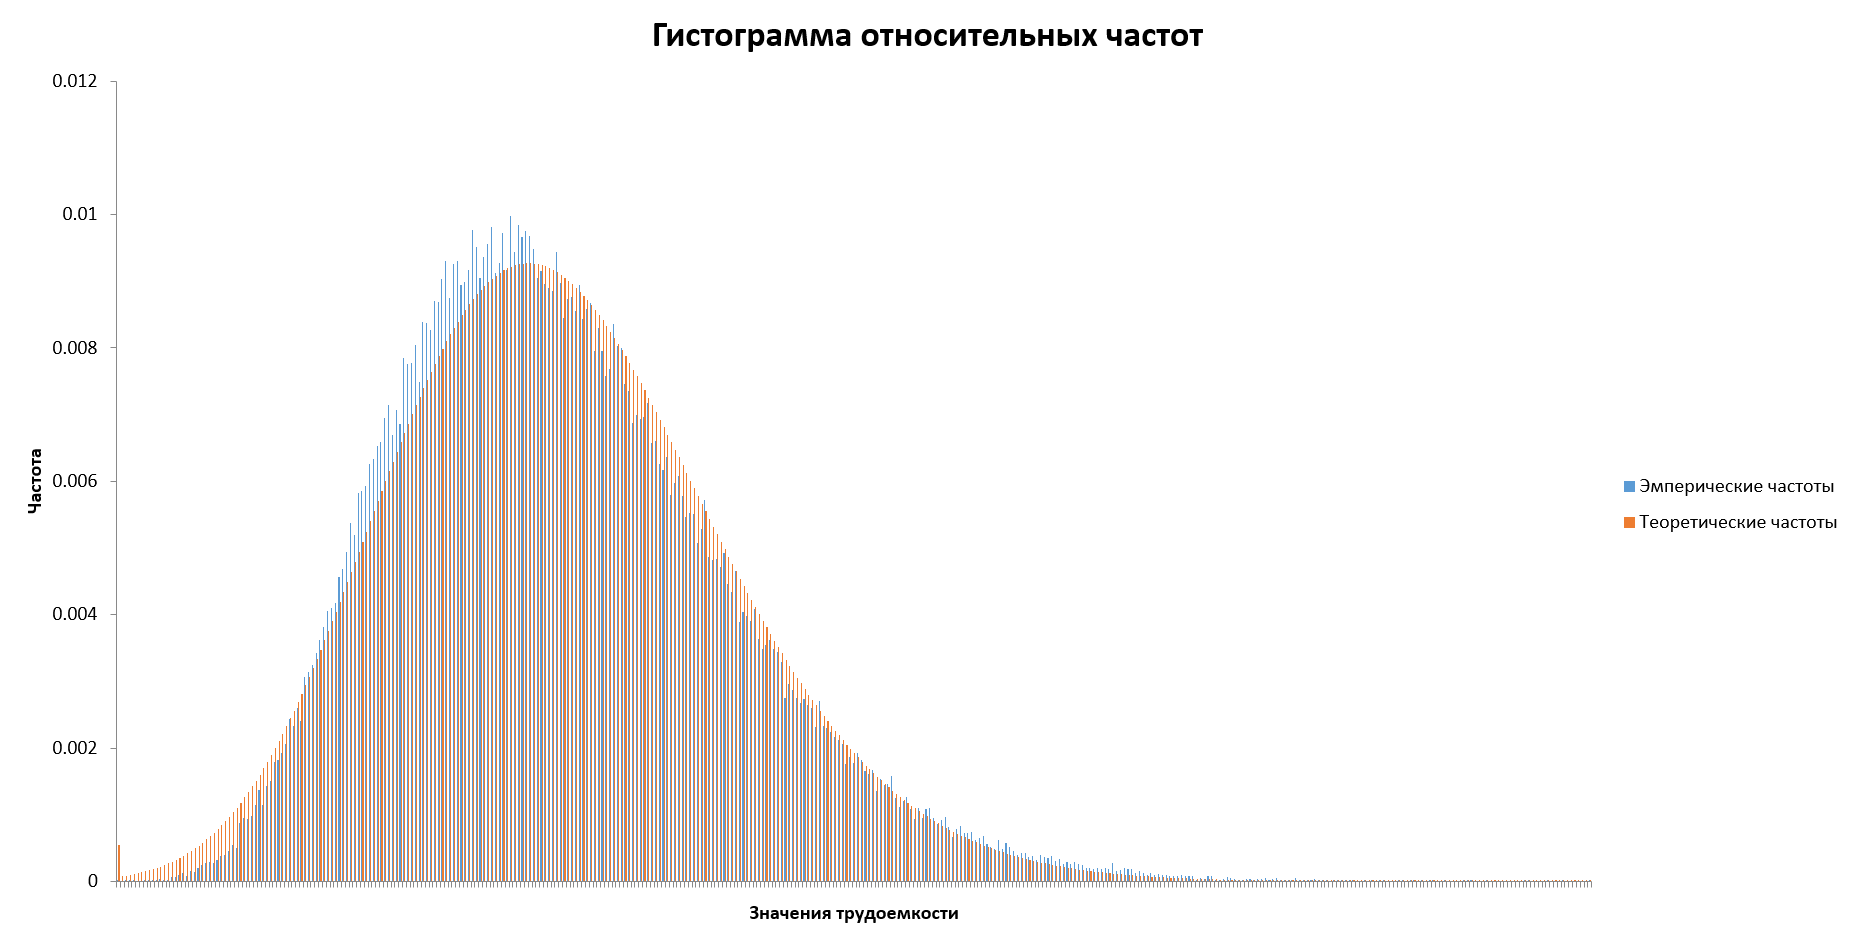
\includegraphics[width=\linewidth]{histogram.png}}
	\caption{теоретические и эмпирические частоты для алгоритма Паллоттино при $n = 80$ с разбиением нормированного сегмента [0, 1] на 387 полусегментов}
	\label{fig:histogram}
\end{figure}

\begin{figure}[!]
	\center{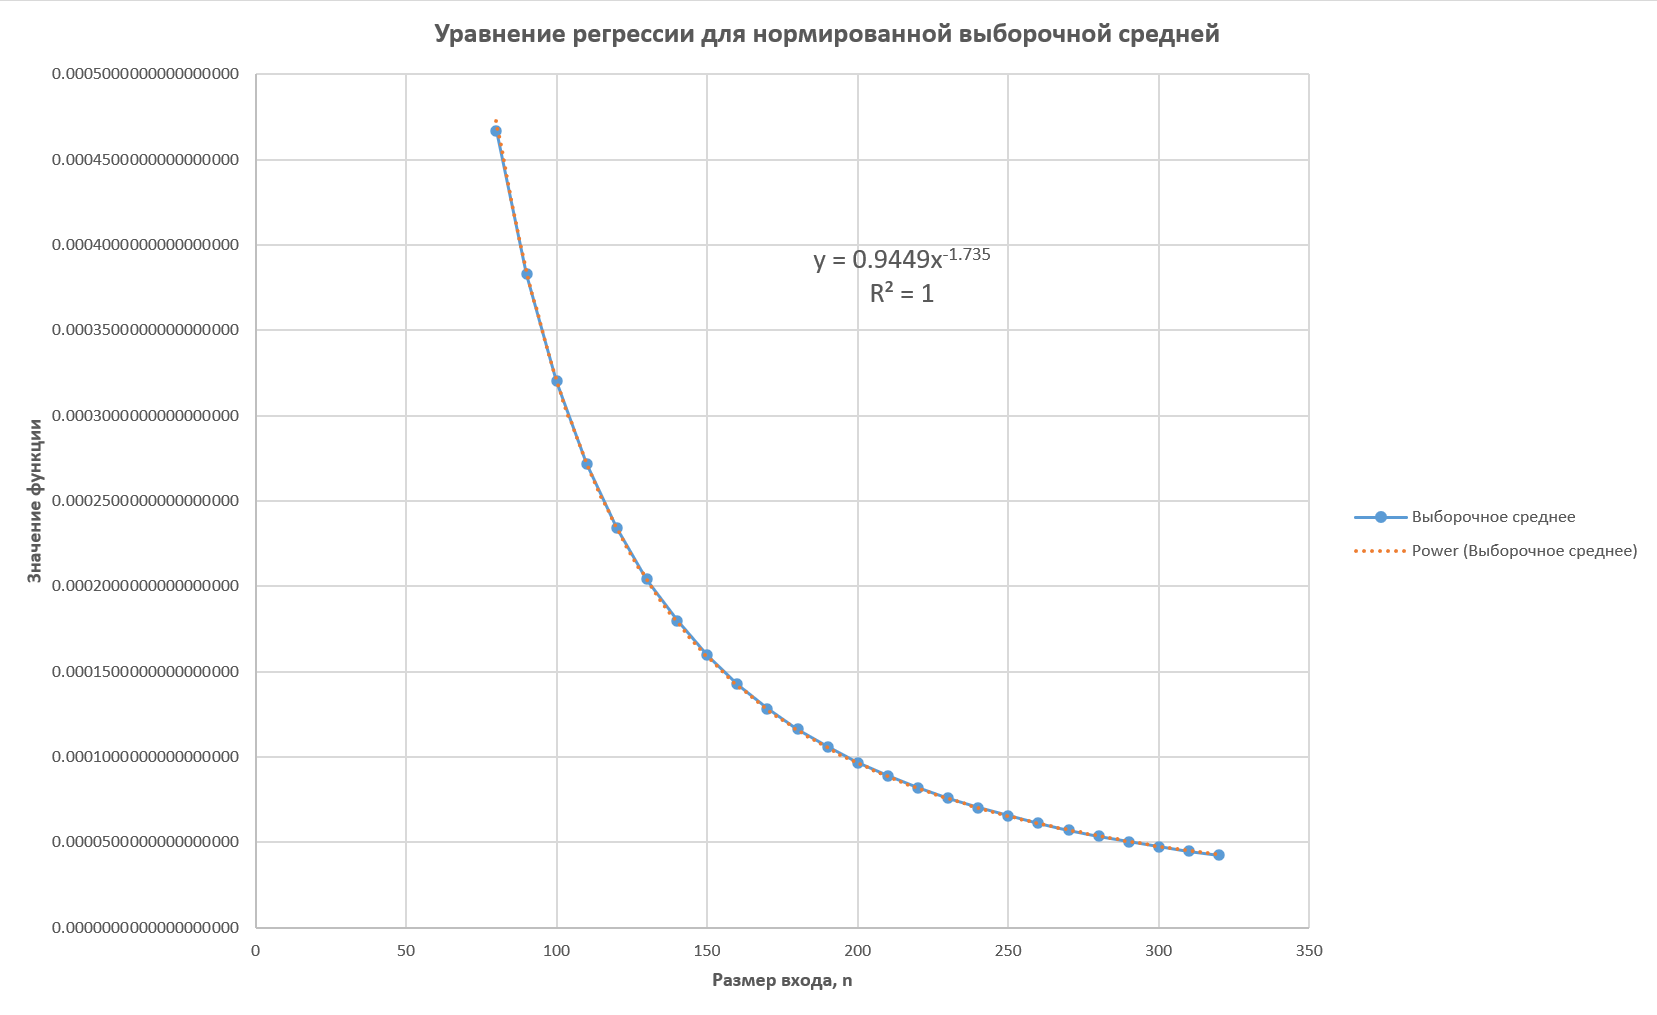
\includegraphics[width=\linewidth]{prediction_mean.png}}
	\caption{экспериментальные данные и уравнение регрессии для нормированной выборочной средней значений трудоемкости алгоритма Паллоттино}
	\label{fig:regression_mean}
\end{figure}

\begin{figure}[!]
	\center{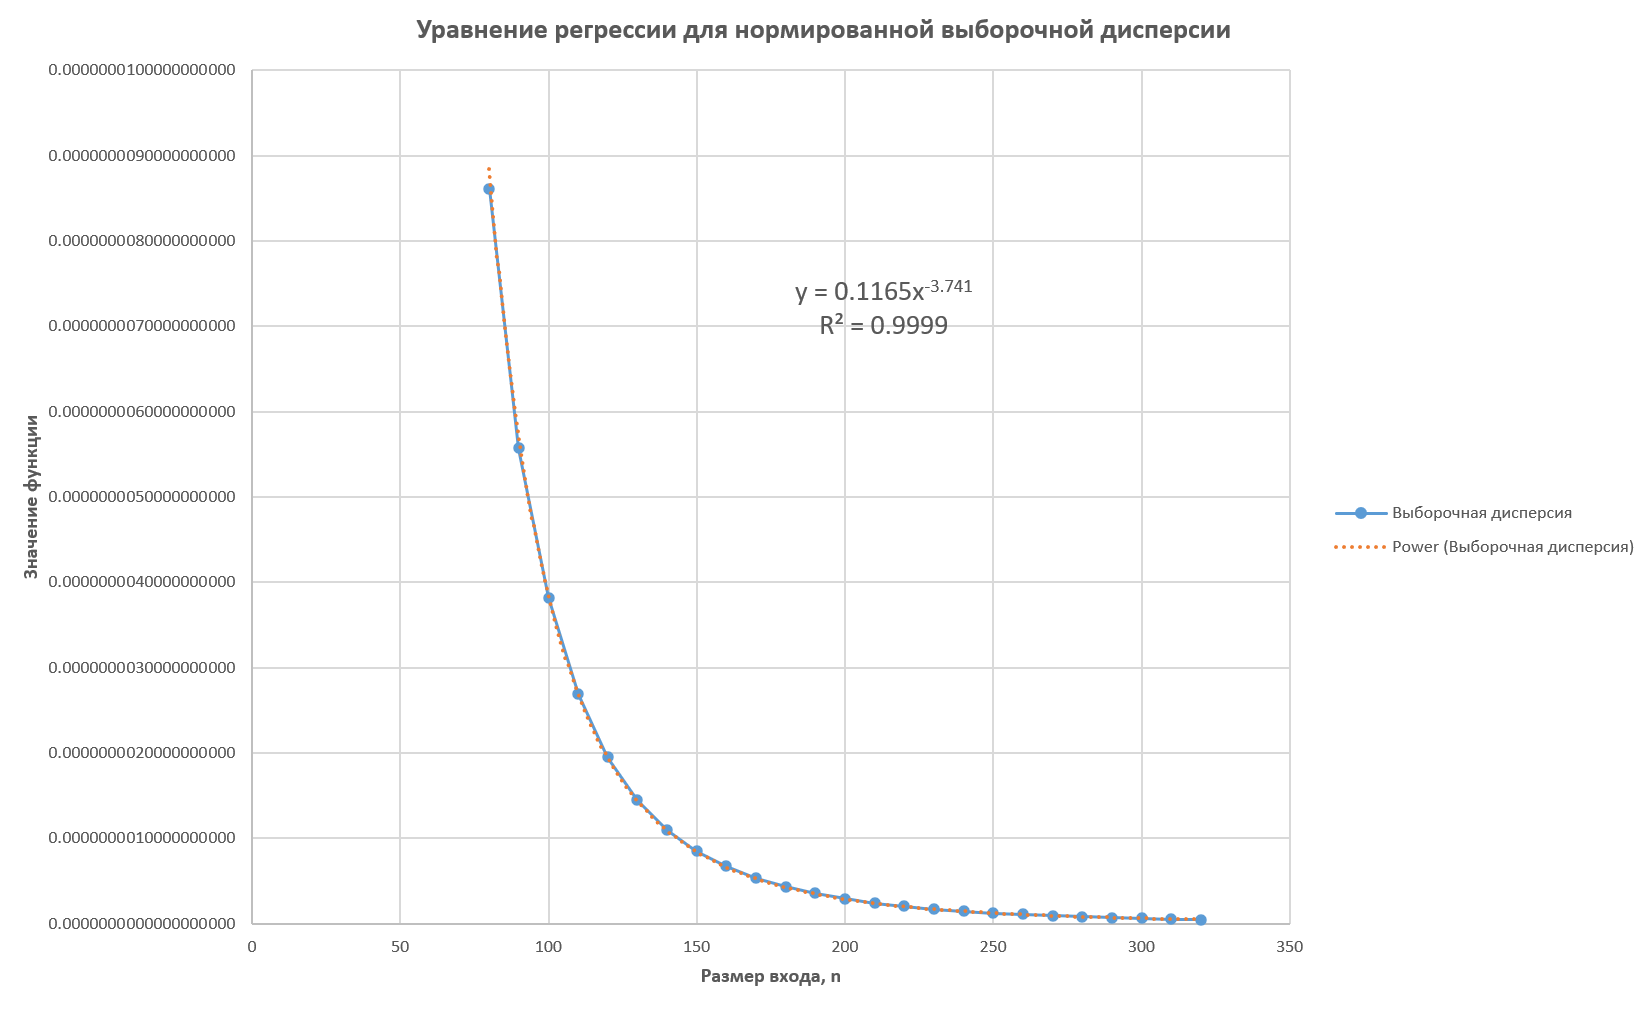
\includegraphics[width=\linewidth]{prediction_variance.png}}
	\caption{экспериментальные данные и уравнение регрессии для нормированной выборочной дисперсии значений трудоемкости алгоритма Паллоттино}
	\label{fig:regression_variance}
\end{figure}

\begin{figure}[!]
	\center{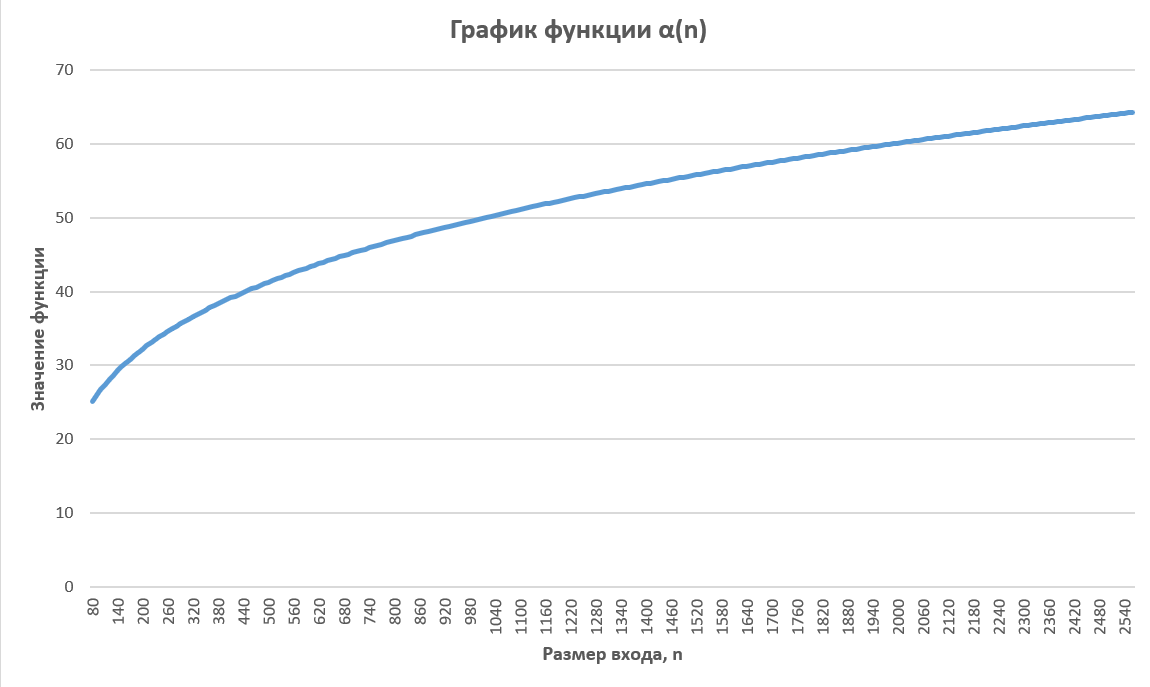
\includegraphics[width=\linewidth]{alpha.png}}
	\caption{график функции $\alpha(n)$~--- параметра $\alpha$ аппроксимирующего бета"=распределения для алгоритма Паллоттино}
	\label{fig:alpha_plot}
\end{figure}

\begin{figure}[!]
	\center{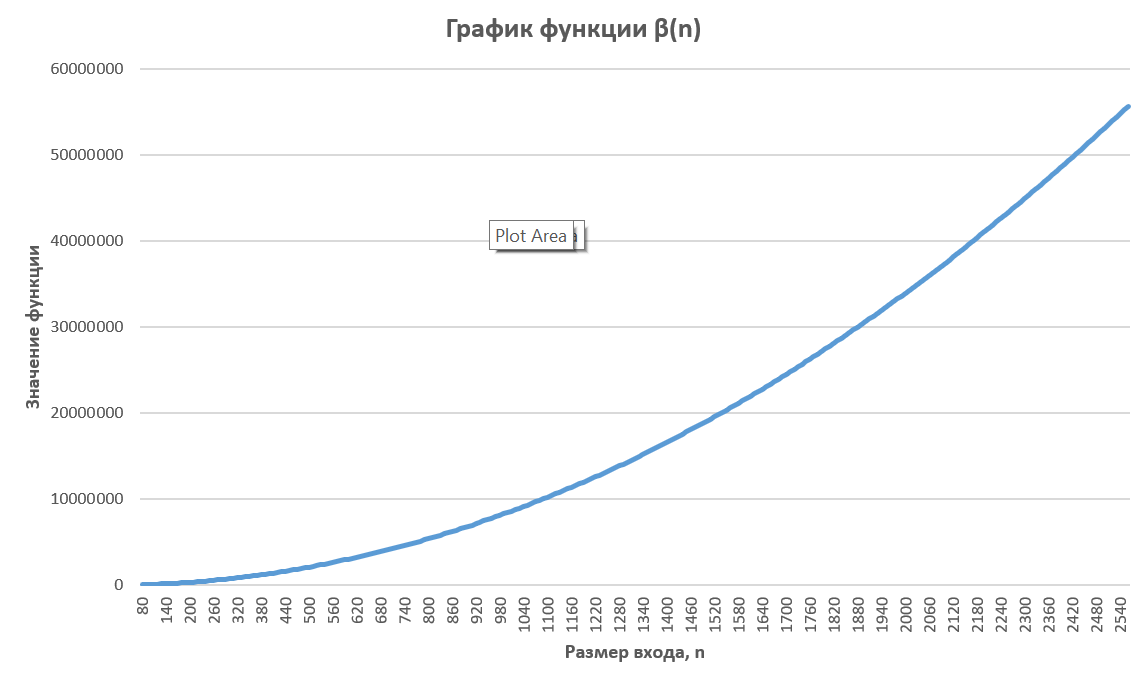
\includegraphics[width=\linewidth]{beta.png}}
	\caption{график функции $\beta(n)$~--- параметра $\beta$ аппроксимирующего бета"=распределения для алгоритма Паллоттино}
	\label{fig:beta_plot}
\end{figure}

\begin{figure}[!]
	\center{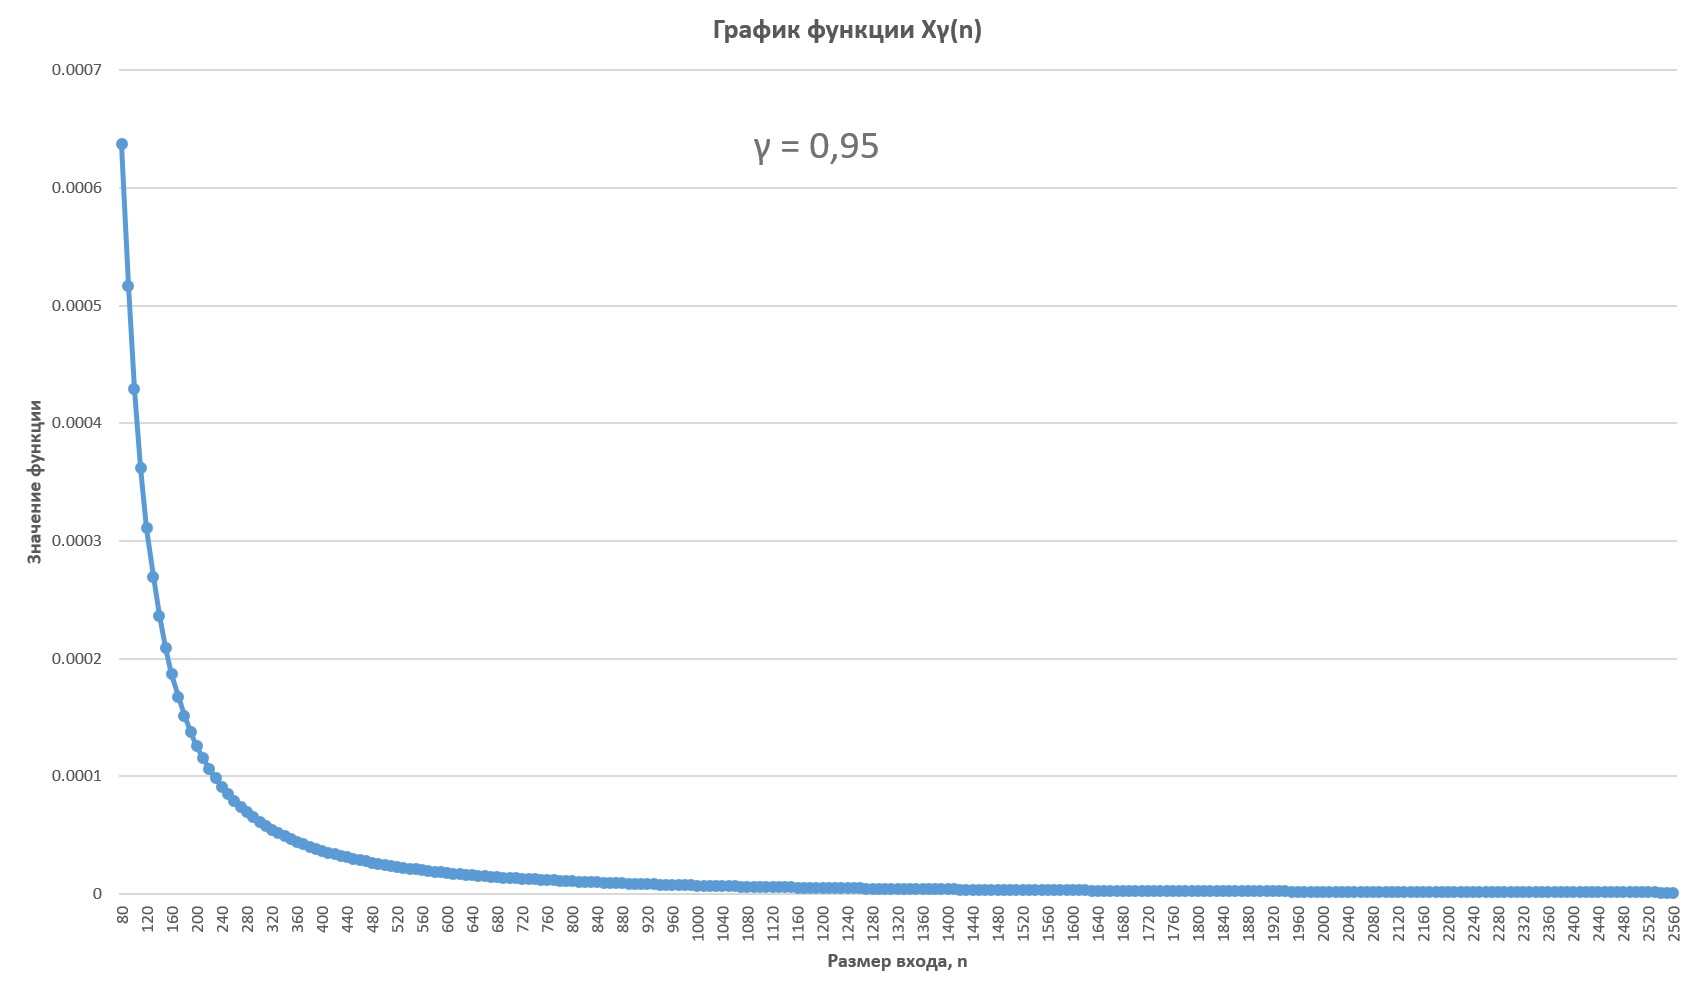
\includegraphics[width=\linewidth]{quantile.png}}
	\caption{график зависимости левого $\gamma$"=квантиля бета"=распределения $x_\gamma(n)$ от длины входа для алгоритма Паллоттино}
	\label{fig:quantile}
\end{figure}

\begin{figure}[!]
	\center{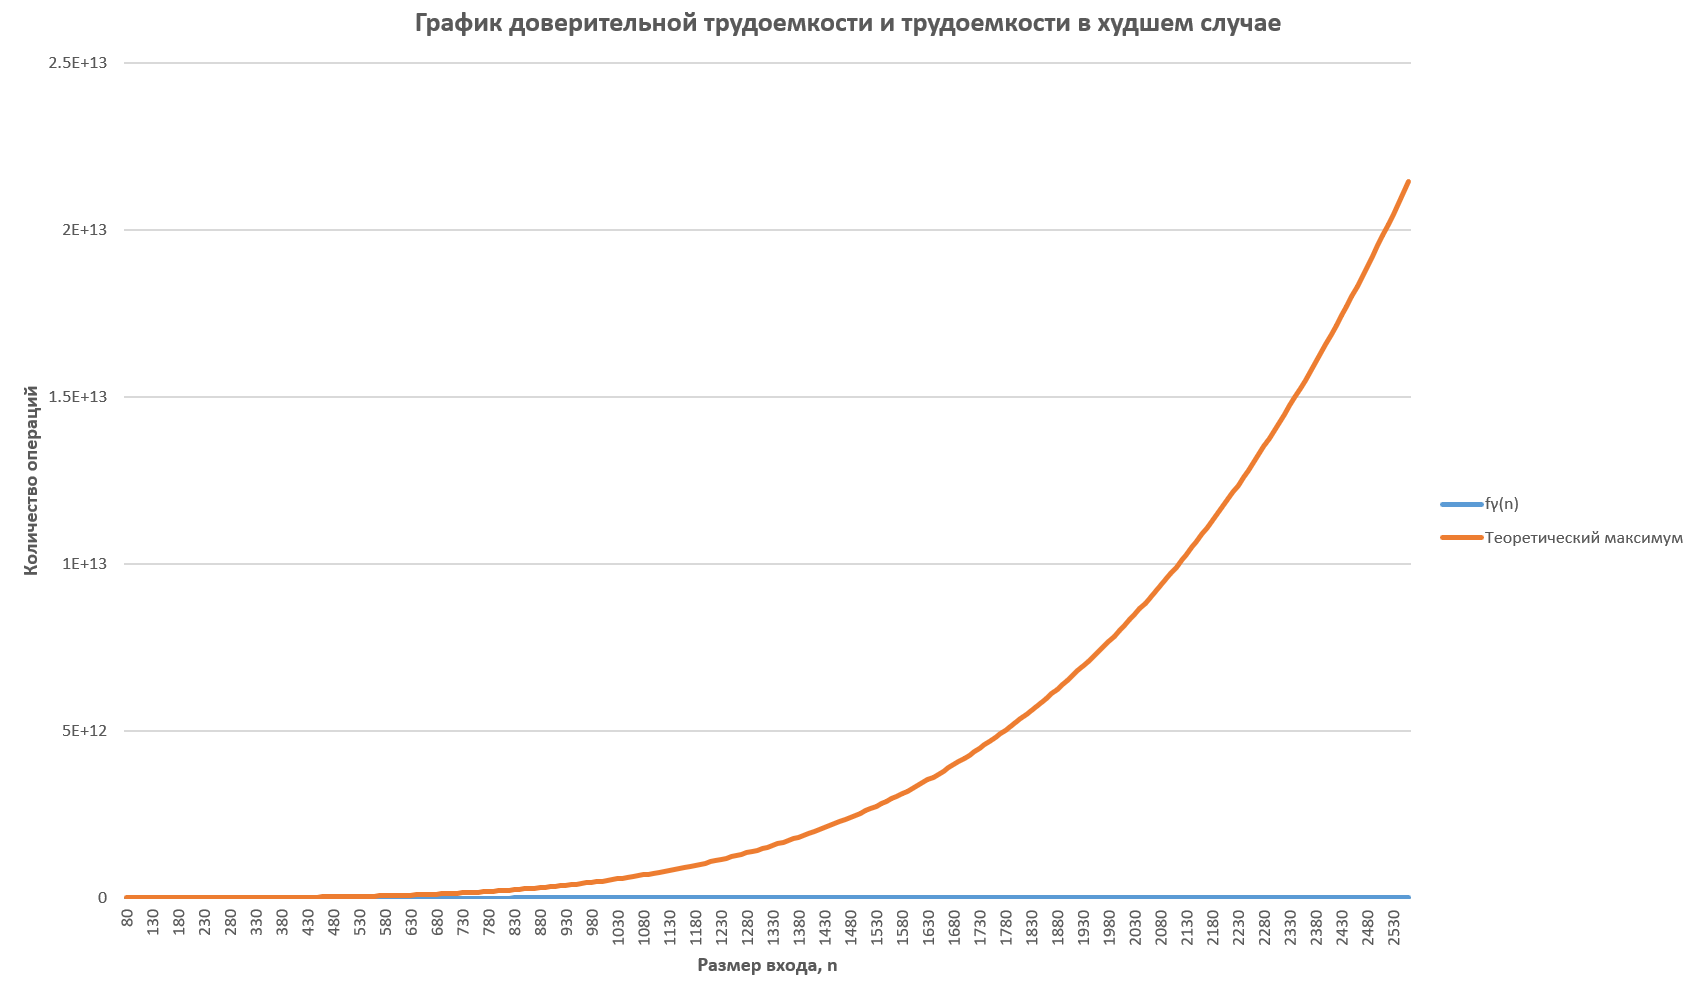
\includegraphics[width=\linewidth]{comparison.png}}
	\caption{график доверительной трудоемкости и трудоемкости в худшем случае для алгоритма Паллоттино}
	\label{fig:comparison_complexities}
\end{figure}

\newpage

%\section{Список литературы} \label{sec:sources}
\begin{thebibliography}{1} \label{sec:sources}

	\bibitem{petrushyn_ulyanov_planning} Петрушин~В.\:Н., Ульянов~М.\:В. Планирование экспериментального исследования трудоемкости алгоритмов на основе бета"=распределения // Информационные технологии и вычислительные системы. 2008. \No~2. С.~81--91.
	
	\bibitem{petrushyn_ulyanov_analysis} Петрушин~В.\:Н., Ульянов~М.\:В., Кривенцов~А.\:С. Доверительная трудоемкость~--- новая оценка качества алгоритмов // Информационные технологии и вычислительные системы. 2009. \No~2. С.~23--37.
		
	\bibitem{dijkstra} Dijkstra~E.\:W. A note on two problems in connexion with graphs // Numer. Math. 1959. Vol.~1. P.~269--271.

	\bibitem{bellman} Bellman~R. On a routing problem // Quart. Appl. Math. 1958. Vol.~16. P.~87--90.
	
	\bibitem{ford} Ford~L.\:R. and Fulkerson~D.\:R. Flows in Networks // Princeton:~Princeton University Press. 1962.
	
	\bibitem{moore} Moore~E.\:F. The shortest path through a maze // Bell Telephone System. Technical publications. 1959. Vol.~3523.
	
	\bibitem{desopo} Pollack~M. and Wiebenson~W. Solutions of the shortest"=route problem – A review // Oper. Res. 8. 1960. P.~224--230.
	
	\bibitem{pape} Pape~U. Implementation and efficiency of Moore"=algorithms for the shortest route problem // Math. Program. 1974. Vol.~7. P.~212--222.
	
	\bibitem{levit_livshits} Левит~Б.\:Ю., Лившиц~В.\:Н. Нелинейные сетевые транспортные задачи // Институт комплексных транспортных проблем. М., Изд-во «Транспорт». 1972. С.~1--144.
	
	\bibitem{pallottino} Pallottino~S. Shortest"=path methods: Complexity, interrelations and new propositions // Networks. 1984. Vol.~14. P.~257--267.

\end{thebibliography}

\end{document}
